% begin module MVT-meaning
\begin{frame}[t]
\begin{theorem}[The Mean Value Theorem]
Let $f$ be a function that is continuous on $[a,b]$ and differentiable on $(a,b)$.
Then there is a number $c$ in $(a,b)$ such that $f'(c) = \frac{f(b)-f(a)}{b-a}$.
\end{theorem}
\begin{columns}[c]
\column{.5\textwidth}
\only<handout:1|2-5>{%
\psset{xunit=1cm, yunit=1cm}
\begin{pspicture}(-5, -5)(5,5)
\psframe*[linecolor=white](-5,-5)(5,5)
\psaxes[ticks=none, labels=none]{<->}(0,0)(-0.5,-0.5)(5.1,4)\tiny
\fcLabels{5.1}{4}
%Function formula: 2-1/3 ((-2+x)^{2})
\psplot[linecolor=\fcColorGraph, plotpoints=1000]{1}{4}{x -2 add 2 exp -0.333333 mul 2 add }
%Function formula: 2-1/3 (x)
\psplot[linecolor=\fcColorTangent, plotpoints=1000]{0.3}{4.5}{x -0.333333 mul 2 add }
\uncover<5->{
%Function formula: 11/4-1/3 (x)
\psplot[linecolor=\fcColorTangent, plotpoints=1000]{0.3}{4.5}{x -0.333333 mul 2.75 add }
\fcFullDot{2.5}{1.916666667}
\psline[linestyle=dashed](2.5, 0)(2.5,1.916666667)
\rput[b](2.5,2.016666667){$(c,f(c))$}
\fcXTick{2.5}
\rput[t](2.5, -0.2){$c$}
}
\fcFullDot{1}{1.666666667}
\rput[tr](1,1.566666667){$(a,f(a))$}
\fcXTick{1}
\rput[t](1, -0.2){$a$}

\fcFullDot{4}{0.666666667}
\rput[tl](4,0.566666667){$(b,f(b))$}
\fcXTick{4}
\rput[t](4, -0.2){$b$}
\end{pspicture}

%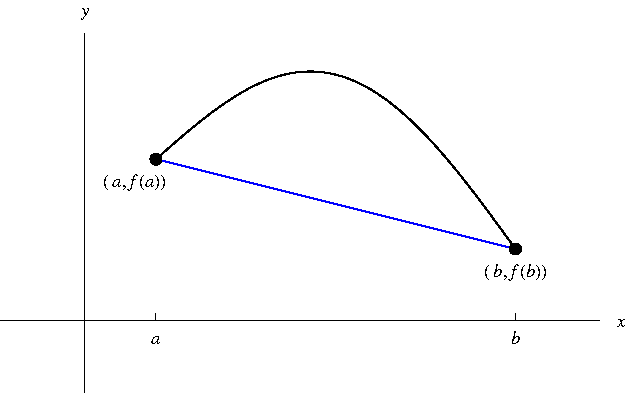
\includegraphics[height=4cm]{maxima-minima/pictures/04-02-mvta.pdf}%
%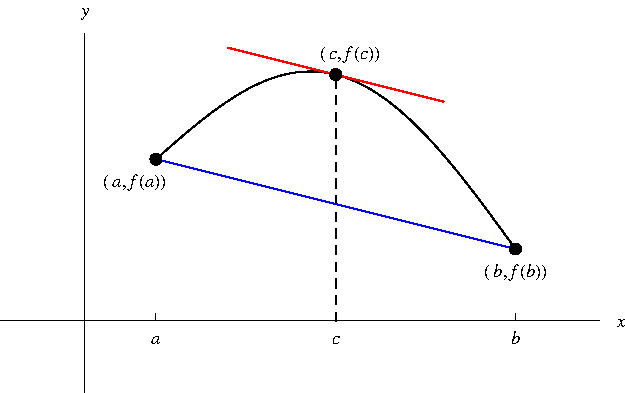
\includegraphics[height=4cm]{maxima-minima/pictures/04-02-mvtb.pdf}%
}%
\only<handout:2| 6->{%
\psset{xunit=1cm, yunit=1cm}
\begin{pspicture}(-5, -5)(5,5)
\psframe*[linecolor=white](-5,-5)(5,5)
\psaxes[ticks=none, labels=none]{<->}(0,0)(-0.5,-0.5)(5.1,4)\tiny
\fcLabels{5.1}{4}

\fcFullDot{0.6}{0.708}
\fcXTick{0.6}
\rput[t](0.6,-0.2){$a$}
\rput[t] (0.6, 0.5){$(a, f(a))$}

\fcFullDot{4.4}{3.292}
\fcXTick{4.4}
\rput[t](4.4,-0.2){$b$}
\rput[b] (4.2, 3.5){$(b, f(b))$}


\fcFullDot{1.403034489}{2.57408}
\fcXTick{1.403034489}
\psline[linestyle=dashed](1.403034489,0)(1.403034489,2.57408)
\rput[t](1.403034489,-0.2){$c_1$}
\rput[b] (1.403034489, 2.87408){$(c_1, f(c_1))$}

\fcFullDot{3.596965511}{1.42592}
\fcXTick{3.596965511}
\psline[linestyle=dashed](3.596965511,0)(3.596965511,1.42592)
\rput[t](3.596965511,-0.2){$c_2$}
\rput[lt] (3.696965511, 1.42){$(c_2, f(c_2))$}

%Function formula: -3+33/4 (x)+1/2 ((x)^{3})-15/4 ((x)^{2})
\psplot[linecolor=\fcColorGraph, plotpoints=1000]{0.6}{4.4}{x 2 exp -3.75 mul x 3 exp 0.5 mul x 8.25 mul -3 add add add }
%Function formula: -25500413687/25000000000+17/25 (x)
\psplot[linecolor=\fcColorTangent, plotpoints=1000]{1.6}{5}{x 0.68 mul -1.02002 add } %Function formula: 40500413687/25000000000+17/25 (x)
\psplot[linecolor=\fcColorTangent, plotpoints=1000]{-0.25}{3}{x 0.68 mul 1.62002 add } %Function formula: 3/10+17/25 (x)
\psplot[linecolor=\fcColorTangent, plotpoints=1000]{-0.25}{5}{x 0.68 mul 0.3 add }
\end{pspicture}
%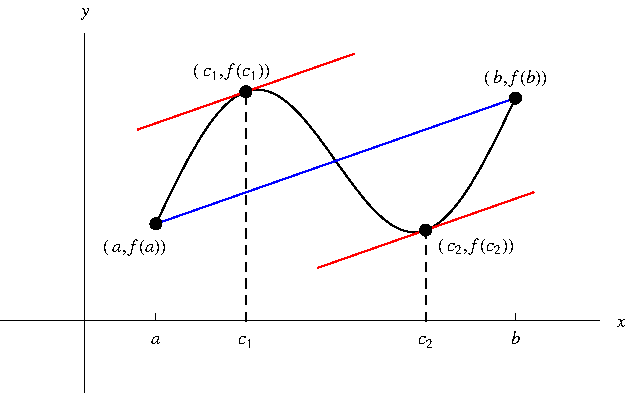
\includegraphics[height=4cm]{maxima-minima/pictures/04-02-mvtc.pdf}%
}%
\column{.5\textwidth}
\begin{itemize}
\item<2->  Consider the secant line from $(a, f(a))$ to $(b, f(b))$.
\item<2-| alert@3-4>  Slope: $m =  \fcAnswer{4}{\frac{f(b)-f(a)}{b-a}.}$
\item<5->  The Mean Value Theorem says that there exists a number $c$ in $(a,b)$ such that the slope of the tangent at $c$ equals $m$.
\item<handout:2| 6->  More than one number is allowed.
\end{itemize}
\end{columns}

\vspace{2cm} %guarantees top alignment of slide
\end{frame}
% end module MVT-meaning
